\documentclass{article}
\usepackage{graphics} 
\usepackage{hyperref}
\usepackage{fixltx2e}
\usepackage{amssymb}
\usepackage{tikz}

\author{Kevin Zollicoffer}
\title{Regression\\Final}
\date{11/04/2013}

% no indents
\setlength\parindent{0pt}

\usepackage{Sweave}
\begin{document}
\maketitle
%\tableofcontents
\Sconcordance{concordance:RegressionFinal.tex:RegressionFinal.Rnw:%
1 14 1 1 0 14 1 1 2 1 0 2 1 12 0 1 2 1 1 1 9 12 0 1 2 5 1 1 2 1 0 2 1 %
28 0 1 1 3 0 1 3 5 0 1 2 8 1 1 2 5 0 1 2 1 1 1 2 1 0 1 1 4 0 1 2 1 1 1 %
2 1 0 3 1 1 2 3 1 1 2 3 1 3 0 1 2 1 5 4 0 1 2 43 0 1 2 8 1 1 2 1 0 1 1 %
38 0 1 1 16 0 1 2 3 1 1 4 3 0 1 1 35 0 1 1 15 0 1 2 3 1 1 3 2 0 1 1 36 %
0 1 2 5 1 1 3 2 0 1 1 33 0 2 1 3 0 1 3 5 0 1 2 9 1 1 2 1 0 3 1 3 0 1 2 %
2 1 1 2 1 0 5 1 3 0 1 2 4 1 1 2 1 0 2 1 5 0 1 3 9 1}


\section*{Introduction}
Regression final assignment using R
\\
\\
The complete source for this assigment is available on Github:
\\
\\
\url{https://github.com/zollie/PASS}

\section*{Problem 5.5}
\begin{Schunk}
\begin{Sinput}
> ubs <- read.csv("~/R/PASS/Regression/RegressionFinal/ubs.csv")
> ubs$Region = factor(ubs$Region)
> head(ubs)
\end{Sinput}
\begin{Soutput}
       City Region DAs DEm DSa Bigmac  Wage Bread  Rice Vac
1 Amsterdam NaWeOc   0   0   0  2.944 4.263 2.303 2.398  26
2    Athens NaWeOc   0   0   0  3.401 3.829 2.565 3.296  22
3  Auckland NaWeOc   0   0   0  2.944 3.786 2.944 2.565  21
4   Bangkok   Asia   1   0   0  3.807 2.653 3.761 3.296   7
5 Barcelona NaWeOc   0   0   0  3.045 4.119 2.833 2.079  23
6   Beijing   Asia   1   0   0  3.784 2.625 3.951 3.434   9
\end{Soutput}
\end{Schunk}

\subsection*{a}
\begin{Schunk}
\begin{Sinput}
> pairs(cbind(ubs$Bigmac, 
+             ubs$DAs, ubs$DEm, ubs$DSa, 
+             ubs$Wage, ubs$Bread, 
+             ubs$Rice, ubs$Vac), 
+       labels=cbind("Bigmac", 
+                    "DAs", "DEm", "DSa", 
+                    "Wage", "Bread", 
+                    "Rice", "Vac"))
\end{Sinput}
\end{Schunk}
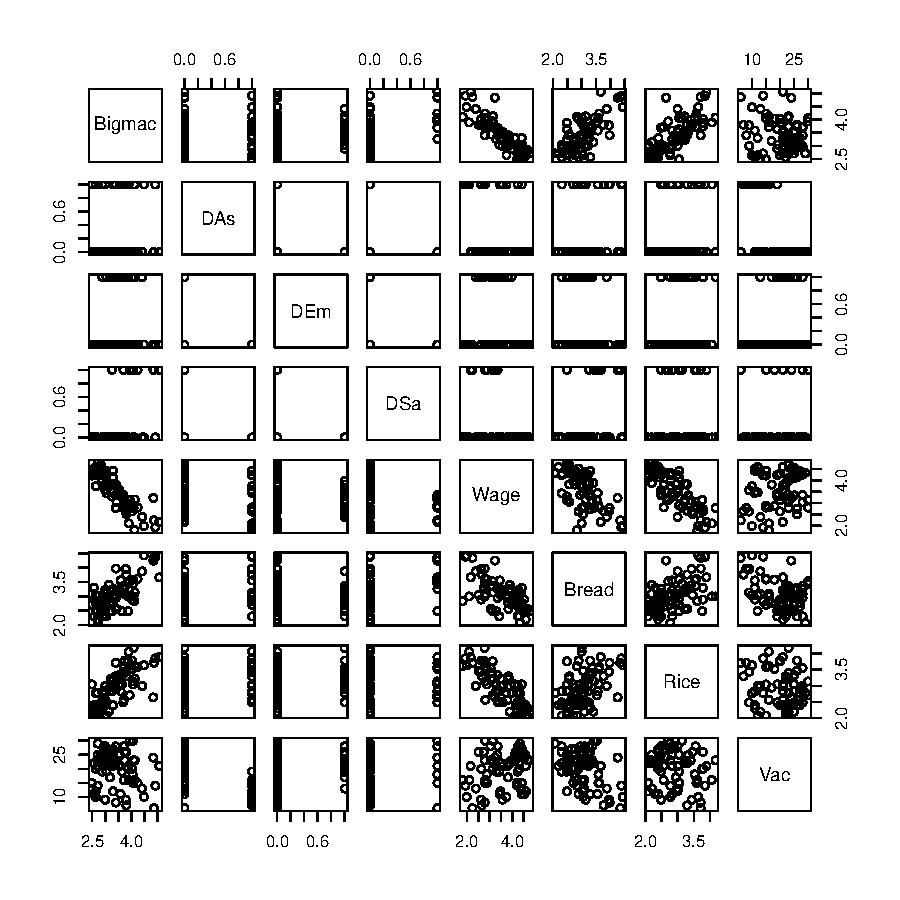
\includegraphics{RegressionFinal-002}

There seems to be clear linear relationships with Wage and Bigmac (negative), Bread and Bigmac, and Rice and Bigmac. The predictive power for Vac of Bigmac is less clear.  
\\\\
There seems to be some correlation between Wage and Bread, and Wage and Rice. 

\subsection*{b}
\begin{Schunk}
\begin{Sinput}
> model_b <- lm(Bigmac ~ DAs+DEm+DSa+Wage+Bread+Rice+Vac, data=ubs)
> stu_b <- rstudent(model_b)
> summary(model_b)
\end{Sinput}
\begin{Soutput}
Call:
lm(formula = Bigmac ~ DAs + DEm + DSa + Wage + Bread + Rice + 
    Vac, data = ubs)

Residuals:
     Min       1Q   Median       3Q      Max 
-0.44853 -0.16851 -0.03561  0.14513  0.63157 

Coefficients:
             Estimate Std. Error t value Pr(>|t|)    
(Intercept)  3.929449   0.631421   6.223 3.99e-08 ***
DAs         -0.207525   0.114411  -1.814   0.0743 .  
DEm         -0.104153   0.094352  -1.104   0.2737    
DSa          0.181246   0.118389   1.531   0.1306    
Wage        -0.576032   0.084254  -6.837 3.37e-09 ***
Bread        0.309707   0.074294   4.169 9.25e-05 ***
Rice         0.102046   0.088928   1.148   0.2554    
Vac          0.015415   0.005814   2.651   0.0101 *  
---
Signif. codes:  0 ‘***’ 0.001 ‘**’ 0.01 ‘*’ 0.05 ‘.’ 0.1 ‘ ’ 1

Residual standard error: 0.2331 on 65 degrees of freedom
Multiple R-squared:  0.8807,	Adjusted R-squared:  0.8678 
F-statistic: 68.54 on 7 and 65 DF,  p-value: < 2.2e-16
\end{Soutput}
\begin{Sinput}
> plot(ubs$Bread, stu_b)
\end{Sinput}
\end{Schunk}
\begin{Schunk}
\begin{Sinput}
> scatter.smooth(ubs$Bread, stu_b, span=.75)
\end{Sinput}
\end{Schunk}
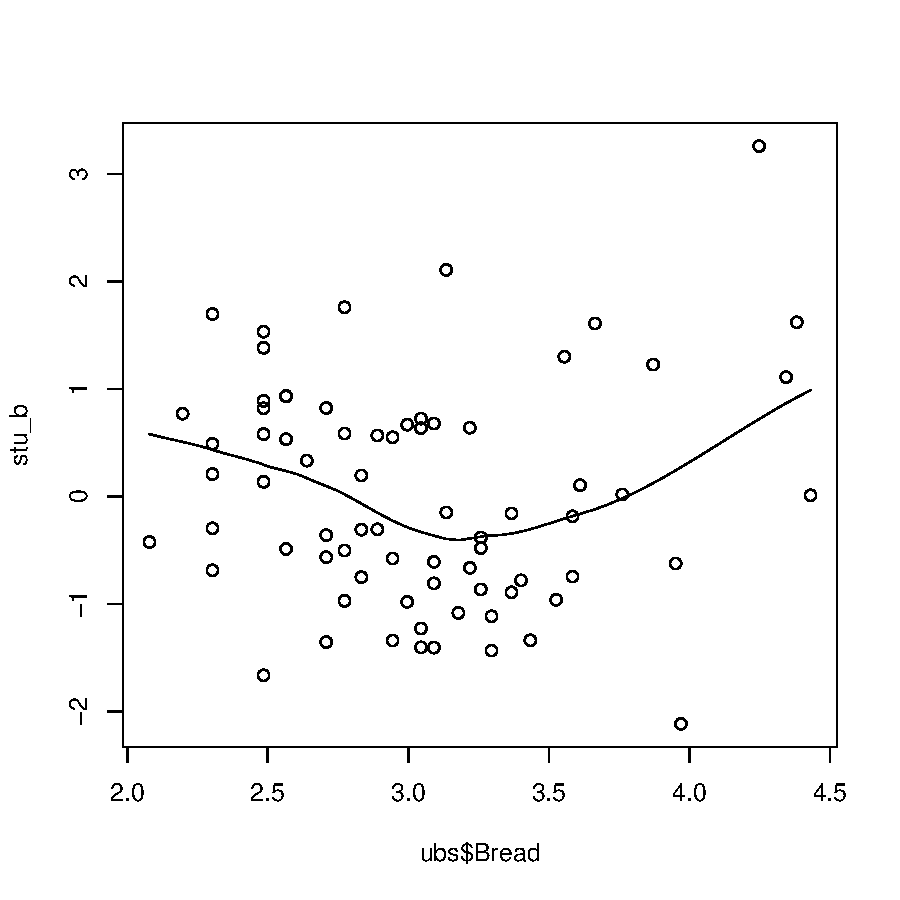
\includegraphics{RegressionFinal-004}
\\\\
The zero mean assumption can be tested with a loess line as above. 
\\\\
The constant variance assumption can be checked by ensuring the studentized residuals are distributed evenly about the mean. That is, they have a mean of 0 and a standard deviation of 1. 
\\\\
The independence assumption can be checked with a quick glance at a residual scatter plot to ensure there are no non-random patterns. 
\\\\
The normailty assumption can be checked with histograms and QQ plots as below.

\begin{Schunk}
\begin{Sinput}
> hist(stu_b)
\end{Sinput}
\end{Schunk}
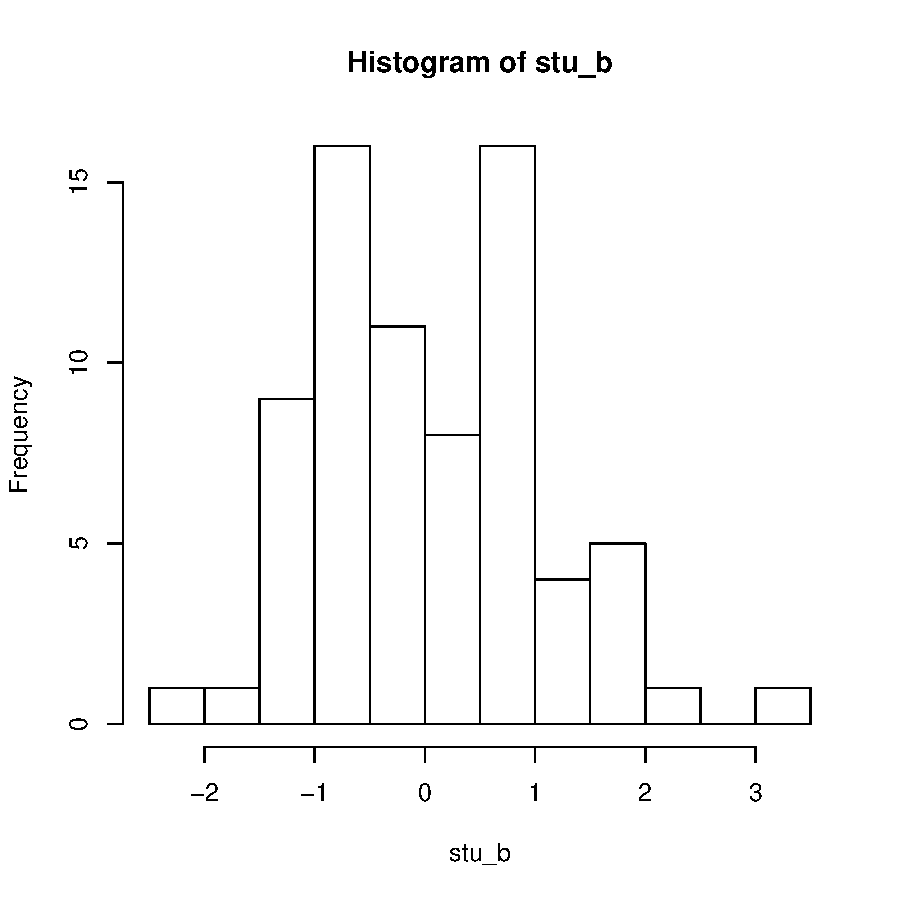
\includegraphics{RegressionFinal-005}

To check the constant vriance assumption we can use a histogram \ldots
\begin{Schunk}
\begin{Sinput}
> qqnorm(stu_b)
> qqline(stu_b)
\end{Sinput}
\end{Schunk}
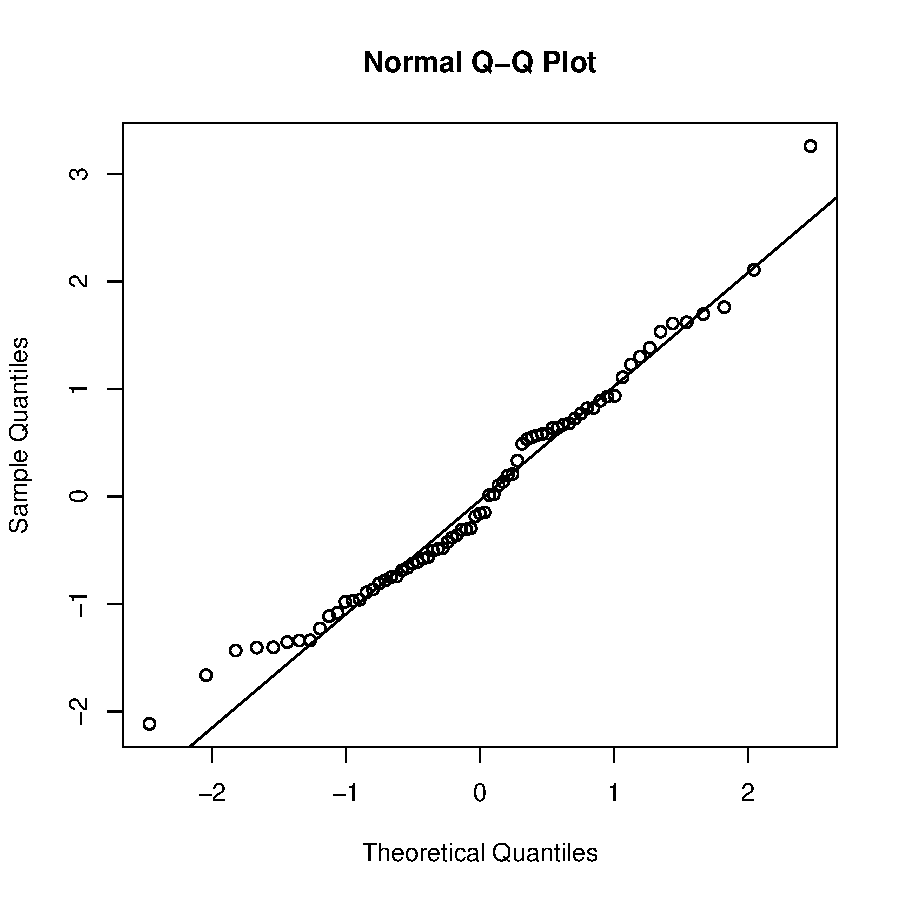
\includegraphics{RegressionFinal-006}

\subsection*{c}
\begin{Schunk}
\begin{Sinput}
> DasWage <- ubs$DAs*ubs$Wage
> DasBread <- ubs$DAs*ubs$Bread
> DasRice <- ubs$DAs*ubs$Rice
> DasVac <- ubs$DAs*ubs$Vac
> DemWage <- ubs$DEm*ubs$Wage
> DemBread <- ubs$DEm*ubs$Bread
> DemRice <- ubs$DEm*ubs$Rice
> DemVac <- ubs$DEm*ubs$Vac
> DsaWage <- ubs$DSa*ubs$Wage
> DsaBread <- ubs$DSa*ubs$Bread
> DsaRice <- ubs$DSa*ubs$Rice
> DsaVac <- ubs$DSa*ubs$Vac
\end{Sinput}
\end{Schunk}

\begin{Schunk}
\begin{Sinput}
> model_c <- lm(Bigmac ~ DAs+DEm+DSa+Wage+Bread+Rice
+               +Vac+DasWage+DasBread+DasRice+DasVac
+               +DemWage+DemBread+DemRice+DemVac+DsaWage
+               +DsaBread+DsaRice+DsaVac, data=ubs)
> summary(model_c)
\end{Sinput}
\begin{Soutput}
Call:
lm(formula = Bigmac ~ DAs + DEm + DSa + Wage + Bread + Rice + 
    Vac + DasWage + DasBread + DasRice + DasVac + DemWage + DemBread + 
    DemRice + DemVac + DsaWage + DsaBread + DsaRice + DsaVac, 
    data = ubs)

Residuals:
     Min       1Q   Median       3Q      Max 
-0.32656 -0.12469 -0.01427  0.10780  0.49710 

Coefficients:
             Estimate Std. Error t value Pr(>|t|)    
(Intercept)  3.683085   0.996793   3.695 0.000522 ***
DAs         -0.738972   1.459567  -0.506 0.614749    
DEm          0.555744   1.383537   0.402 0.689532    
DSa         -0.984978   2.907659  -0.339 0.736134    
Wage        -0.478023   0.154255  -3.099 0.003106 ** 
Bread        0.082348   0.107430   0.767 0.446765    
Rice         0.221956   0.122558   1.811 0.075804 .  
Vac          0.022065   0.007127   3.096 0.003131 ** 
DasWage     -0.103942   0.188635  -0.551 0.583933    
DasBread     0.567501   0.183594   3.091 0.003176 ** 
DasRice     -0.463639   0.202251  -2.292 0.025882 *  
DasVac       0.054241   0.021818   2.486 0.016104 *  
DemWage     -0.051375   0.214087  -0.240 0.811278    
DemBread     0.208266   0.175752   1.185 0.241303    
DemRice     -0.011267   0.203540  -0.055 0.956064    
DemVac      -0.045066   0.015387  -2.929 0.005005 ** 
DsaWage     -0.130008   0.460941  -0.282 0.779005    
DsaBread     0.690651   0.189595   3.643 0.000614 ***
DsaRice     -0.160711   0.384538  -0.418 0.677684    
DsaVac      -0.007723   0.013443  -0.575 0.568045    
---
Signif. codes:  0 ‘***’ 0.001 ‘**’ 0.01 ‘*’ 0.05 ‘.’ 0.1 ‘ ’ 1

Residual standard error: 0.1903 on 53 degrees of freedom
Multiple R-squared:  0.9351,	Adjusted R-squared:  0.9119 
F-statistic: 40.21 on 19 and 53 DF,  p-value: < 2.2e-16
\end{Soutput}
\end{Schunk}

The 3 interactions with largest p-value are \ldots
\begin{enumerate}
\item DemWage
\item DemRice
\item DsaWage
\end{enumerate}

\subsection*{d}
\begin{Schunk}
\begin{Sinput}
> model_d <- lm(Bigmac ~ DAs+DEm+DSa+Wage+Bread+Rice+Vac+DasWage+DasBread+DasRice+DasVac+DemBread+DemVac+DsaBread+DsaRice+DsaVac, data=ubs)
> summary(model_d)
\end{Sinput}
\begin{Soutput}
Call:
lm(formula = Bigmac ~ DAs + DEm + DSa + Wage + Bread + Rice + 
    Vac + DasWage + DasBread + DasRice + DasVac + DemBread + 
    DemVac + DsaBread + DsaRice + DsaVac, data = ubs)

Residuals:
     Min       1Q   Median       3Q      Max 
-0.32589 -0.12401 -0.01427  0.10882  0.49611 

Coefficients:
             Estimate Std. Error t value Pr(>|t|)    
(Intercept)  3.873477   0.707313   5.476 1.06e-06 ***
DAs         -0.929363   1.256451  -0.740  0.46259    
DEm          0.282447   0.565201   0.500  0.61922    
DSa         -1.752632   0.898657  -1.950  0.05615 .  
Wage        -0.511492   0.100893  -5.070 4.66e-06 ***
Bread        0.075781   0.102562   0.739  0.46306    
Rice         0.209768   0.092579   2.266  0.02735 *  
Vac          0.022123   0.006832   3.238  0.00203 ** 
DasWage     -0.070473   0.146160  -0.482  0.63157    
DasBread     0.574068   0.177613   3.232  0.00206 ** 
DasRice     -0.451451   0.182008  -2.480  0.01616 *  
DasVac       0.054183   0.021215   2.554  0.01340 *  
DemBread     0.224488   0.158454   1.417  0.16210    
DemVac      -0.045118   0.013701  -3.293  0.00172 ** 
DsaBread     0.714585   0.166165   4.300 6.89e-05 ***
DsaRice     -0.076633   0.179529  -0.427  0.67112    
DsaVac      -0.007269   0.012880  -0.564  0.57475    
---
Signif. codes:  0 ‘***’ 0.001 ‘**’ 0.01 ‘*’ 0.05 ‘.’ 0.1 ‘ ’ 1

Residual standard error: 0.1854 on 56 degrees of freedom
Multiple R-squared:  0.935,	Adjusted R-squared:  0.9164 
F-statistic: 50.33 on 16 and 56 DF,  p-value: < 2.2e-16
\end{Soutput}
\begin{Sinput}
> anova(model_d, model_c)
\end{Sinput}
\begin{Soutput}
Analysis of Variance Table

Model 1: Bigmac ~ DAs + DEm + DSa + Wage + Bread + Rice + Vac + DasWage + 
    DasBread + DasRice + DasVac + DemBread + DemVac + DsaBread + 
    DsaRice + DsaVac
Model 2: Bigmac ~ DAs + DEm + DSa + Wage + Bread + Rice + Vac + DasWage + 
    DasBread + DasRice + DasVac + DemWage + DemBread + DemRice + 
    DemVac + DsaWage + DsaBread + DsaRice + DsaVac
  Res.Df    RSS Df Sum of Sq      F Pr(>F)
1     56 1.9243                           
2     53 1.9198  3 0.0045205 0.0416 0.9886
\end{Soutput}
\end{Schunk}

The p-value of .9886 > .05 therefore we cannot reject $H_0$. We can remove the 3 interactions with the largest p-value as statistically $DemWage=DemRice=DsaWage=0$

\subsection*{e}
\begin{Schunk}
\begin{Sinput}
> model_e <- lm(Bigmac ~ DAs+DEm+DSa+Wage+Bread
+               +Rice+Vac+DasBread+DasRice+DasVac
+               +DemBread+DemVac+DsaBread, data=ubs)
> summary(model_e)
\end{Sinput}
\begin{Soutput}
Call:
lm(formula = Bigmac ~ DAs + DEm + DSa + Wage + Bread + Rice + 
    Vac + DasBread + DasRice + DasVac + DemBread + DemVac + DsaBread, 
    data = ubs)

Residuals:
     Min       1Q   Median       3Q      Max 
-0.31559 -0.11941 -0.00559  0.10736  0.49558 

Coefficients:
             Estimate Std. Error t value Pr(>|t|)    
(Intercept)  4.110961   0.553962   7.421 5.23e-10 ***
DAs         -1.512860   0.632105  -2.393 0.019894 *  
DEm          0.212223   0.542260   0.391 0.696935    
DSa         -2.219990   0.508840  -4.363 5.23e-05 ***
Wage        -0.541401   0.071295  -7.594 2.67e-10 ***
Bread        0.065805   0.098576   0.668 0.507019    
Rice         0.189425   0.073788   2.567 0.012809 *  
Vac          0.020716   0.005185   3.995 0.000182 ***
DasBread     0.608153   0.163987   3.709 0.000463 ***
DasRice     -0.394569   0.137903  -2.861 0.005830 ** 
DasVac       0.057814   0.019994   2.892 0.005358 ** 
DemBread     0.226347   0.154589   1.464 0.148451    
DemVac      -0.042906   0.012967  -3.309 0.001600 ** 
DsaBread     0.729123   0.153530   4.749 1.35e-05 ***
---
Signif. codes:  0 ‘***’ 0.001 ‘**’ 0.01 ‘*’ 0.05 ‘.’ 0.1 ‘ ’ 1

Residual standard error: 0.1816 on 59 degrees of freedom
Multiple R-squared:  0.9342,	Adjusted R-squared:  0.9197 
F-statistic: 64.47 on 13 and 59 DF,  p-value: < 2.2e-16
\end{Soutput}
\begin{Sinput}
> anova(model_e, model_d)
\end{Sinput}
\begin{Soutput}
Analysis of Variance Table

Model 1: Bigmac ~ DAs + DEm + DSa + Wage + Bread + Rice + Vac + DasBread + 
    DasRice + DasVac + DemBread + DemVac + DsaBread
Model 2: Bigmac ~ DAs + DEm + DSa + Wage + Bread + Rice + Vac + DasWage + 
    DasBread + DasRice + DasVac + DemBread + DemVac + DsaBread + 
    DsaRice + DsaVac
  Res.Df    RSS Df Sum of Sq      F Pr(>F)
1     59 1.9464                           
2     56 1.9243  3  0.022104 0.2144  0.886
\end{Soutput}
\end{Schunk}

The p-value of .886 > .05 therefore we cannot reject $H_0$. We can remove the 3 interactions considered here. 

\subsection*{f}
\begin{Schunk}
\begin{Sinput}
> model_f <- lm(Bigmac ~ DAs+DEm+DSa+Wage+Bread+Rice+
+                 Vac+DasBread+DasRice+DasVac+DemBread+DemVac+DsaBread, data=ubs)
> summary(model_f)
\end{Sinput}
\begin{Soutput}
Call:
lm(formula = Bigmac ~ DAs + DEm + DSa + Wage + Bread + Rice + 
    Vac + DasBread + DasRice + DasVac + DemBread + DemVac + DsaBread, 
    data = ubs)

Residuals:
     Min       1Q   Median       3Q      Max 
-0.31559 -0.11941 -0.00559  0.10736  0.49558 

Coefficients:
             Estimate Std. Error t value Pr(>|t|)    
(Intercept)  4.110961   0.553962   7.421 5.23e-10 ***
DAs         -1.512860   0.632105  -2.393 0.019894 *  
DEm          0.212223   0.542260   0.391 0.696935    
DSa         -2.219990   0.508840  -4.363 5.23e-05 ***
Wage        -0.541401   0.071295  -7.594 2.67e-10 ***
Bread        0.065805   0.098576   0.668 0.507019    
Rice         0.189425   0.073788   2.567 0.012809 *  
Vac          0.020716   0.005185   3.995 0.000182 ***
DasBread     0.608153   0.163987   3.709 0.000463 ***
DasRice     -0.394569   0.137903  -2.861 0.005830 ** 
DasVac       0.057814   0.019994   2.892 0.005358 ** 
DemBread     0.226347   0.154589   1.464 0.148451    
DemVac      -0.042906   0.012967  -3.309 0.001600 ** 
DsaBread     0.729123   0.153530   4.749 1.35e-05 ***
---
Signif. codes:  0 ‘***’ 0.001 ‘**’ 0.01 ‘*’ 0.05 ‘.’ 0.1 ‘ ’ 1

Residual standard error: 0.1816 on 59 degrees of freedom
Multiple R-squared:  0.9342,	Adjusted R-squared:  0.9197 
F-statistic: 64.47 on 13 and 59 DF,  p-value: < 2.2e-16
\end{Soutput}
\end{Schunk}
$H_0: DemBread=0$
$H_a: D_{Em}\neq0$
\\\\
$.1484 > .05$ therefore we do not reject $H_0$

\subsection*{g}
\begin{Schunk}
\begin{Sinput}
> model_g <- lm(Bigmac ~ DAs+DEm+DSa+Wage+Bread+Rice+
+ Vac+DasBread+DasRice+DasVac+DemVac+DsaBread, data=ubs)
> summary(model_g)
\end{Sinput}
\begin{Soutput}
Call:
lm(formula = Bigmac ~ DAs + DEm + DSa + Wage + Bread + Rice + 
    Vac + DasBread + DasRice + DasVac + DemVac + DsaBread, data = ubs)

Residuals:
     Min       1Q   Median       3Q      Max 
-0.27016 -0.12943  0.00022  0.10108  0.51102 

Coefficients:
             Estimate Std. Error t value Pr(>|t|)    
(Intercept)  3.861757   0.532170   7.257 9.12e-10 ***
DAs         -1.207924   0.602473  -2.005 0.049487 *  
DEm          0.876811   0.299504   2.928 0.004821 ** 
DSa         -1.991641   0.488946  -4.073 0.000138 ***
Wage        -0.547934   0.071831  -7.628 2.11e-10 ***
Bread        0.154348   0.078586   1.964 0.054162 .  
Rice         0.195452   0.074372   2.628 0.010889 *  
Vac          0.021595   0.005199   4.153 0.000105 ***
DasBread     0.515727   0.152786   3.375 0.001297 ** 
DasRice     -0.406481   0.138969  -2.925 0.004856 ** 
DasVac       0.056577   0.020165   2.806 0.006759 ** 
DemVac      -0.043681   0.013079  -3.340 0.001446 ** 
DsaBread     0.641239   0.142652   4.495 3.24e-05 ***
---
Signif. codes:  0 ‘***’ 0.001 ‘**’ 0.01 ‘*’ 0.05 ‘.’ 0.1 ‘ ’ 1

Residual standard error: 0.1834 on 60 degrees of freedom
Multiple R-squared:  0.9318,	Adjusted R-squared:  0.9182 
F-statistic: 68.36 on 12 and 60 DF,  p-value: < 2.2e-16
\end{Soutput}
\begin{Sinput}
> stu_g <- rstudent(model_g)
> plot(ubs$Bread, stu_g)
\end{Sinput}
\end{Schunk}
\begin{Schunk}
\begin{Sinput}
> scatter.smooth(ubs$Bread, stu_g, span=.75)
\end{Sinput}
\end{Schunk}
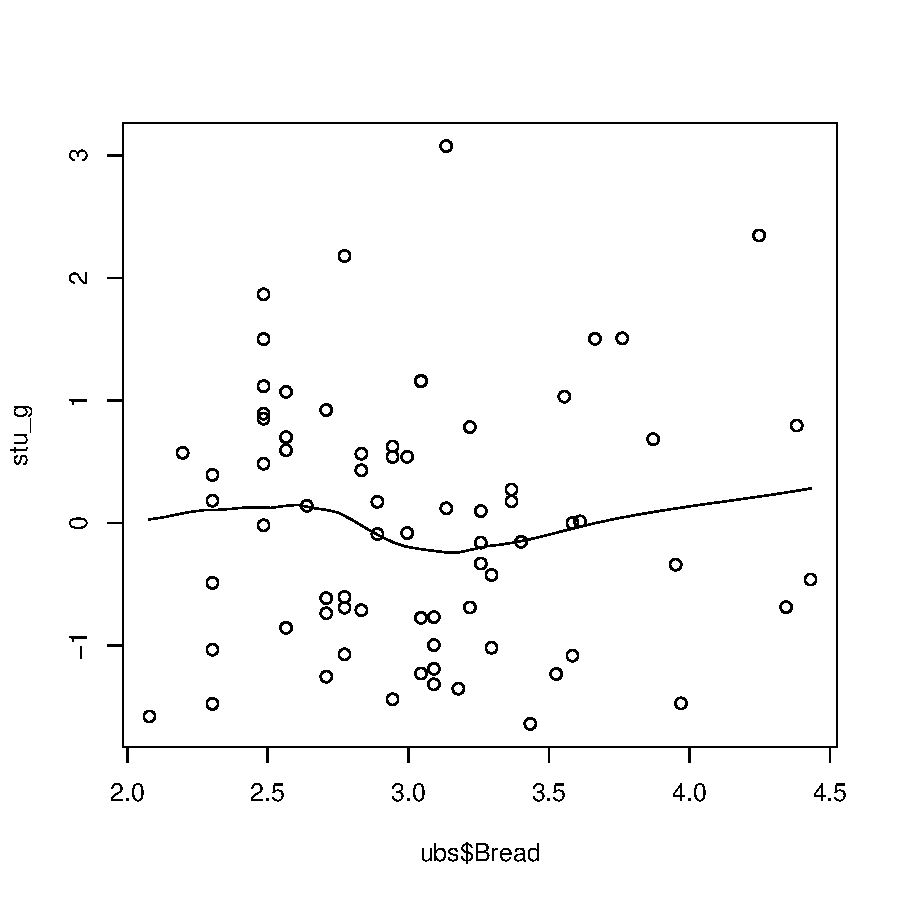
\includegraphics{RegressionFinal-013}

The zero mean regression assumption now appears met. 

\subsection*{h}
$\hat{Bigmac}=3.861757-1.2709D_{As}+.8768D_{Em}-1.99.16D_{Sa}-.5479Wage+.15348Bread+.195452Rice+.021595Vac+.515727DasBread-.406481DasRice+.056577DasVac-.043681DemVac+.641239DsaBread$

\subsection*{i}
Yes, the economist is correct. The coefficient for Wage is negative meaning as Wage increases $\hat{Bigmac}$ decreases all else held constant. 

\subsection*{j}
\begin{Schunk}
\begin{Sinput}
> mWage <- mean(ubs$Wage)
> mBread <- mean(ubs$Bread)
> mRice <- mean(ubs$Rice)
> mVac <- mean(ubs$Vac)
\end{Sinput}
\end{Schunk}

$\hat{Bigmac}=3.861757-1.2709D_{As}+.8768D_{Em}-1.99.16D_{Sa}-mWage*Wage+.15348*Bread+mRice*Rice+mVac*Vac+.15348*DasBread-mRice*DasRice+mVac*DasVac-mVac*DemVac+.15348*DsaBread$
\\
\begin{Schunk}
\begin{Sinput}
> DasBread0 <- DasBread[ubs$DAs==0]
> DasBread1 <- DasBread[ubs$DAs==1]
> DsaBread0 <- DsaBread[ubs$DSa==0]
> DsaBread1 <- DsaBread[ubs$DSa==1]
> DasRice0 <- DasRice[ubs$DAs==0]
> DasRice1 <- DasRice[ubs$DAs==1]
\end{Sinput}
\end{Schunk}



\it{**I am having trouble producing the predictor effect plots below}

\begin{Schunk}
\begin{Sinput}
> plot(ubs$Bread, DasBread, type="n")
> lines(sort(ubs$Bread[ubs$DasBread==0]), DasBread0[order(ubs$Bread[ubs$DasBread==0])])
> lines(sort(ubs$Bread[ubs$DasBread==1]), DasBread1[order(ubs$Bread[ubs$DasBread==1])])
> 
\end{Sinput}
\end{Schunk}
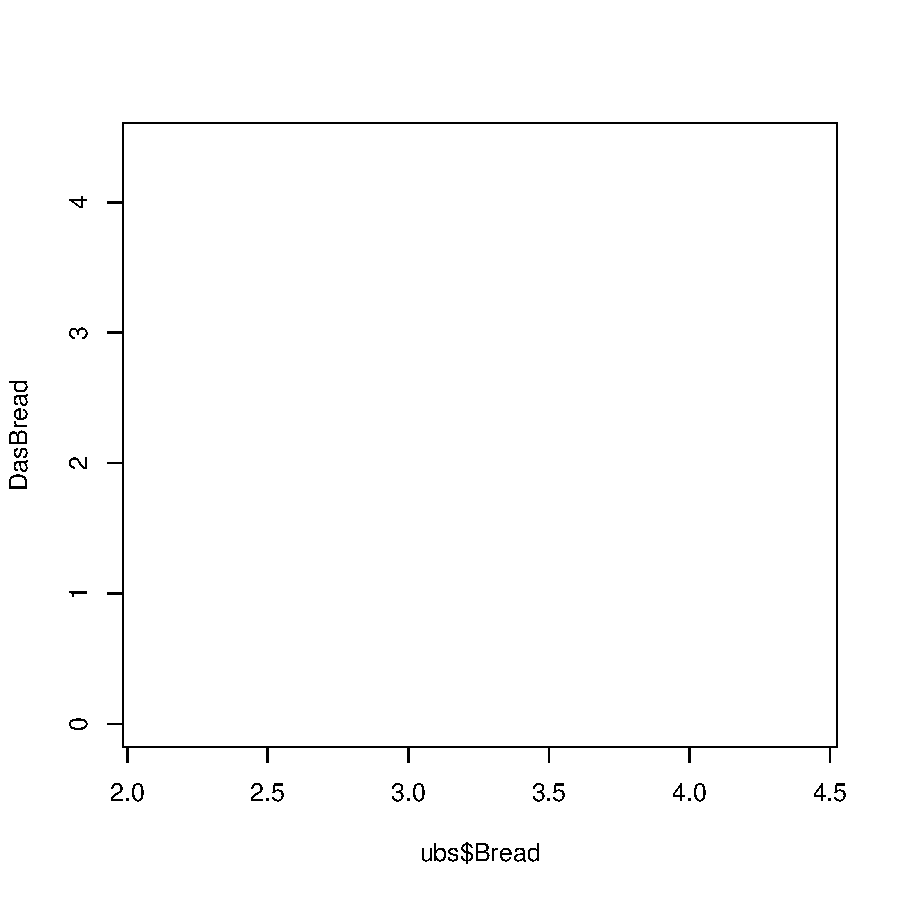
\includegraphics{RegressionFinal-016}

\subsection*{k}
$\hat{Bigmac}=3.861757-1.2709D_{As}+.8768D_{Em}-1.99.16D_{Sa}-mWage*Wage+mBread*Bread+.195452*Rice+mVac*Vac+mBread*DasBread-.195452*DasRice+mVac*DasVac-mVac*DemVac+mBread*DsaBread$


\subsection*{i}
$\hat{Bigmac}=3.861757-1.2709D_{As}+.8768D_{Em}-1.99.16D_{Sa}-mWage*Wage+mBread*Bread+mRice*Rice+.021595*Vac+mBread*DasBread-mRice*DasRice+.021595*DasVac-.021595*DemVac+mBread*DsaBread$


\end{document}
